% ============================================================
% METHODS SECTION
% ============================================================

\section{Methods}\label{sec:methods}

We describe the experimental setup including the gym-sepsis simulation environment, offline and online RL algorithms, LEG interpretability analysis, and evaluation protocol.

% ============================================================
\subsection{Environment and Data}\label{sec:methods:env}

\subsubsection{Gym-Sepsis Simulator}

We use Gym-Sepsis \citep{raghu2017sepsis_drl}, an RL simulator for ICU sepsis treatment trained on MIMIC-III data \citep{johnson2016mimic3}.

At each timestep, the state is a 46-dimensional vector spanning laboratory values such as lactate, creatinine, and platelet count, vital signs such as blood pressure, heart rate, and SpO$_2$, demographics including age, gender, and race, clinical severity scores including SOFA, LODS, SIRS, qSOFA, and Elixhauser, and treatment status including mechanical ventilation and blood culture. The SOFA score \citep{vincent1996sofa} ranges from 0 to 24, with higher values indicating greater organ dysfunction. We use SOFA for severity stratification in Section~\ref{sec:methods:eval}.

The action space is discrete with 24 actions indexed from 0 to 23, derived from a $5 \times 5$ grid over IV fluid and vasopressor dosage bins. The environment implements the mapping $a = \min(5 \times \text{IV\_bin} + \text{VP\_bin}, 23)$, where IV\_bin and VP\_bin are in $\{0, 1, 2, 3, 4\}$, effectively capping the maximum combined dosage at action 23.

Episodes span ICU stays with 4-hour timesteps until discharge or death. We use a sparse reward structure defined as:
\begin{equation}
r_t = \begin{cases}
+15 & \text{if terminal state with patient survival (discharge)} \\
-15 & \text{if terminal state with patient death} \\
0 & \text{for all intermediate timesteps}
\end{cases}
\label{eq:reward}
\end{equation}
where $r_t$ denotes the reward at timestep $t$, and $t = T$ indicates the terminal state of an episode.

\subsubsection{Offline Training Dataset}

We generated an offline dataset of 2,105 episodes with approximately 20K transitions using a heuristic policy based on clinical guidelines \citep{rhodes2017ssc, seymour2017sepsis_criteria}, achieving 94.6\% survival. All episodes were used for training without held-out validation or test sets from the offline data. Performance evaluation was conducted by running trained policies on 500 newly sampled episodes in the gym-sepsis simulator as described in Section~\ref{sec:methods:baselines}.

% ============================================================
\subsection{Algorithms}\label{sec:methods:algos}

We compare 3 offline RL algorithms representing different learning paradigms: Behavior Cloning for supervised learning, Conservative Q-Learning for offline Q-learning, and Deep Q-Network as online RL adapted for offline evaluation. All algorithms use the same neural network architecture for fair comparison, a 3-layer multilayer perceptron with hidden dimensions of 256, 256, and 128 with ReLU activations.

\subsubsection{Behavior Cloning (BC)}

Behavior Cloning treats offline RL as a supervised learning problem, training a policy to imitate the behavioral policy by minimizing the negative log-likelihood of observed actions \citep{pomerleau1991bc}. Given a dataset $\mathcal{D} = \{(s_i, a_i)\}_{i=1}^N$ of state-action pairs, BC learns a policy $\pi_{\theta}(a|s)$ by solving:
\begin{equation}
\theta^* = \arg\min_{\theta} -\frac{1}{N} \sum_{i=1}^N \log \pi_{\theta}(a_i | s_i)
\label{eq:bc}
\end{equation}
where $\theta$ represents the policy network parameters, $N$ is the total number of state-action pairs in the dataset, $s_i$ and $a_i$ are the state and action from the $i$-th sample, and $\pi_{\theta}(a_i | s_i)$ is the probability of selecting action $a_i$ given state $s_i$ under policy $\pi_{\theta}$.

BC is computationally efficient and stable but suffers from distribution shift when the learned policy encounters states not well-represented in the offline dataset \citep{ross2010dagger}.

We use d3rlpy's DiscreteBCConfig with batch size 1,024, learning rate $1 \times 10^{-3}$ with Adam optimizer, training for 50,000 gradient steps over 10 epochs with 5,000 steps per epoch.

\subsubsection{Conservative Q-Learning (CQL)}

Conservative Q-Learning \citep{kumar2020cql} is an offline RL algorithm that learns a conservative Q-function to avoid overestimation on out-of-distribution actions. CQL augments the standard Bellman error with a conservatism penalty that pushes down Q-values for unseen actions while pushing up Q-values for actions in the dataset:
\begin{equation}
\min_Q \alpha \cdot \mathbb{E}_{s \sim \mathcal{D}} \left[ \log \sum_a \exp Q(s, a) - \mathbb{E}_{a \sim \pi_\beta} Q(s, a) \right] + \frac{1}{2} \mathbb{E}_{(s,a,r,s') \sim \mathcal{D}} \left[ (Q(s,a) - \mathcal{T}^\pi Q(s,a))^2 \right]
\label{eq:cql}
\end{equation}
where $Q(s,a)$ is the learned Q-function representing expected cumulative reward for taking action $a$ in state $s$, $\alpha$ is a hyperparameter controlling the strength of the conservatism penalty, $\mathcal{D}$ is the offline dataset, $\pi_\beta$ is the behavioral policy that generated the offline data, and $\mathcal{T}^\pi$ is the Bellman operator defined as $\mathcal{T}^\pi Q(s,a) = r + \gamma \mathbb{E}_{s' \sim P}[\max_{a'} Q(s', a')]$ with discount factor $\gamma$.

The conservatism penalty encourages the learned Q-function to assign lower values to actions that were not taken by the behavioral policy, reducing the risk of selecting suboptimal actions due to Q-value overestimation. The policy is derived as $\pi(s) = \arg\max_a Q(s, a)$.

We use d3rlpy's DiscreteCQLConfig with batch size 1,024, learning rate $3 \times 10^{-4}$ with Adam optimizer, $\alpha = 1.0$, target network updates every 2,000 steps, training for 200,000 gradient steps.

\subsubsection{Deep Q-Network (DQN)}

Deep Q-Network \citep{mnih2015dqn} is a foundational deep RL algorithm that combines Q-learning with deep neural networks. DQN uses 2 key techniques for stability. Experience replay stores transitions in a replay buffer and samples mini-batches for training. A target network $Q_{\theta^-}$ is periodically synchronized with the main network $Q_\theta$ to stabilize Q-value targets.

The Q-function is updated to minimize the temporal difference error:
\begin{equation}
\mathcal{L}(\theta) = \mathbb{E}_{(s,a,r,s') \sim \mathcal{D}} \left[ \left( Q_\theta(s,a) - \left( r + \gamma \max_{a'} Q_{\theta^-}(s', a') \right) \right)^2 \right]
\label{eq:dqn}
\end{equation}
where $\mathcal{L}(\theta)$ is the loss function parameterized by network weights $\theta$, $(s,a,r,s')$ denotes a transition tuple consisting of current state $s$, action $a$, reward $r$, and next state $s'$, $Q_\theta$ is the main Q-network, $Q_{\theta^-}$ is the target Q-network with delayed parameters $\theta^-$, and $\gamma \in [0,1]$ is the discount factor.

The policy is derived greedily as $\pi(s) = \arg\max_a Q_\theta(s, a)$, with $\epsilon$-greedy exploration during training where exploration rate $\epsilon$ is annealed from 1.0 to 0.05.

We use the Stable-Baselines3 library for DQN training. Unlike BC and CQL which train offline on the fixed 2,105-episode dataset, DQN was trained online by interacting with the Gym-Sepsis simulator and accumulating experience in a replay buffer of size 100,000. This reflects DQN's original design as an online RL algorithm \citep{mnih2015dqn}. We include DQN as a foundational baseline representing vanilla Q-learning without offline-specific modifications like CQL's conservatism penalty or architectural innovations like attention mechanisms and residual connections in DDQN variants. This creates a hybrid methodological status where DQN is trained online like DDQN-Attention/Residual and SAC but lacks their architectural enhancements, while being evaluated offline like BC and CQL without their offline training safeguards. Section~\ref{sec:discussion:limitations} discusses the implications of this design choice for interpreting DQN's results. All algorithms are evaluated identically on 500 newly sampled episodes from the gym-sepsis simulator, distinct from the 2,105 training episodes, without further policy updates, ensuring fair performance and interpretability comparison at deployment time.

DQN uses batch size 256, learning rate $1 \times 10^{-4}$ with Adam optimizer, target network updates every 1,000 steps, $\epsilon$-greedy exploration from 1.0 to 0.05, training for 100,000 timesteps.

\subsubsection{Online RL Algorithms}\label{sec:methods:algos:online}

To provide a comprehensive comparison between offline and online RL paradigms, we also evaluate 3 state-of-the-art online RL algorithms with architectural innovations, implemented by collaborator Y. Ding. Unlike the offline methods above, these algorithms train by interacting with the Gym-Sepsis simulator, collecting 1 million timesteps of experience through exploration. This comparison illuminates the performance-safety trade-off. Online methods can explore beyond the behavioral policy's distribution but require environment access during training, a significant constraint in clinical settings where patient safety prohibits trial-and-error learning.

\paragraph{Double DQN with Attention (DDQN-Attention).}
This algorithm extends Double DQN \citep{vanHasselt2016double_dqn} with a multi-head self-attention mechanism in the encoder network. Double DQN addresses Q-value overestimation by decoupling action selection and evaluation. The main network selects the best action while the target network evaluates it. The attention layer allows the model to dynamically weight different state features based on their relevance to the current decision:
\begin{equation}
h_t = \text{MultiHeadAttention}(s_t, s_t, s_t) + s_t
\label{eq:attention}
\end{equation}
where $h_t$ is the hidden representation at timestep $t$, $s_t$ is the input state vector, and the term $+ s_t$ represents the residual connection that helps gradient flow during backpropagation. The MultiHeadAttention function takes query, key, and value inputs (all set to $s_t$ for self-attention). The attention mechanism computes scaled dot-product attention across 4 parallel heads, each learning different feature correlations. The encoder uses 2 hidden layers of 256 and 128 units respectively, with the attention layer inserted after the first hidden layer to capture high-level feature interactions.

\paragraph{Double DQN with Residual Connections (DDQN-Residual).}
This variant incorporates deep residual networks \citep{he2016deep} to enable training of deeper Q-networks without gradient vanishing. The architecture uses 3 hidden layers of 256 units each with skip connections between layers:
\begin{equation}
h_{l+1} = \sigma(\text{LayerNorm}(W_l h_l + b_l + h_{l}'))
\label{eq:residual}
\end{equation}
where $h_l$ is the hidden representation at layer $l$, $h_{l+1}$ is the output of layer $l+1$, $\sigma$ denotes the ReLU activation function, $\text{LayerNorm}$ performs layer normalization, $W_l \in \mathbb{R}^{d \times d}$ and $b_l \in \mathbb{R}^d$ are learnable weight matrix and bias vector for layer $l$, and $h_{l}'$ represents the skip connection input that preserves gradient information during backpropagation. Layer normalization stabilizes training by normalizing activations within each layer. The residual architecture is hypothesized to learn more complex value functions by decomposing Q-value estimation into a base value plus incremental adjustments.

\paragraph{Soft Actor-Critic (SAC).}
SAC \citep{haarnoja2018soft} is a maximum entropy RL algorithm that optimizes both expected return and policy entropy, encouraging exploration and robustness. The objective function is:
\begin{equation}
J(\pi) = \mathbb{E}_{\tau \sim \pi}\left[\sum_t r(s_t, a_t) + \alpha \mathcal{H}(\pi(\cdot|s_t))\right]
\label{eq:sac}
\end{equation}
where $J(\pi)$ is the objective function to be maximized, $\tau$ denotes a trajectory sampled from policy $\pi$, $r(s_t, a_t)$ is the reward received for taking action $a_t$ in state $s_t$ at timestep $t$, $\mathcal{H}(\pi(\cdot|s_t)) = -\sum_a \pi(a|s_t) \log \pi(a|s_t)$ is the entropy of the policy at state $s_t$, and $\alpha > 0$ is a temperature parameter that balances exploitation (maximizing reward) and exploration (maximizing entropy). We use the discrete action space variant of SAC with a residual encoder architecture of 3 layers with 256 units and skip connections. The temperature $\alpha$ is automatically tuned during training using a dual gradient descent approach \citep{haarnoja2018soft_applications}, starting from $\alpha = 0.2$ and adjusting to maintain a target entropy equal to 95\% of the maximum entropy $\log(24)$ for the 24-action space.

\paragraph{Training Details.}
All 3 online RL algorithms were trained with 1,000,000 environment interaction steps using experience replay buffers of size 100,000. Training used batch size 256, learning rate $3 \times 10^{-4}$ with Adam optimizer, and target network soft updates with $\tau = 0.005$. Exploration for DDQN variants used $\epsilon$-greedy with $\epsilon$ annealed from 1.0 to 0.05 over the first 100,000 steps. Unlike offline methods which require only the pre-collected dataset, these algorithms necessitate access to the simulator during training, a key distinction when considering deployment in clinical settings where patient safety prohibits exploratory interventions.

Figure \ref{fig:training-convergence} shows the training convergence curves for all algorithms. Offline methods BC and CQL converge rapidly within 50,000 gradient steps on the fixed dataset, while online methods require approximately 500,000 simulator interactions to reach stable performance. DQN exhibits slower convergence than the enhanced online methods, reflecting its lack of architectural innovations.

\begin{figure}[htbp]
\centering
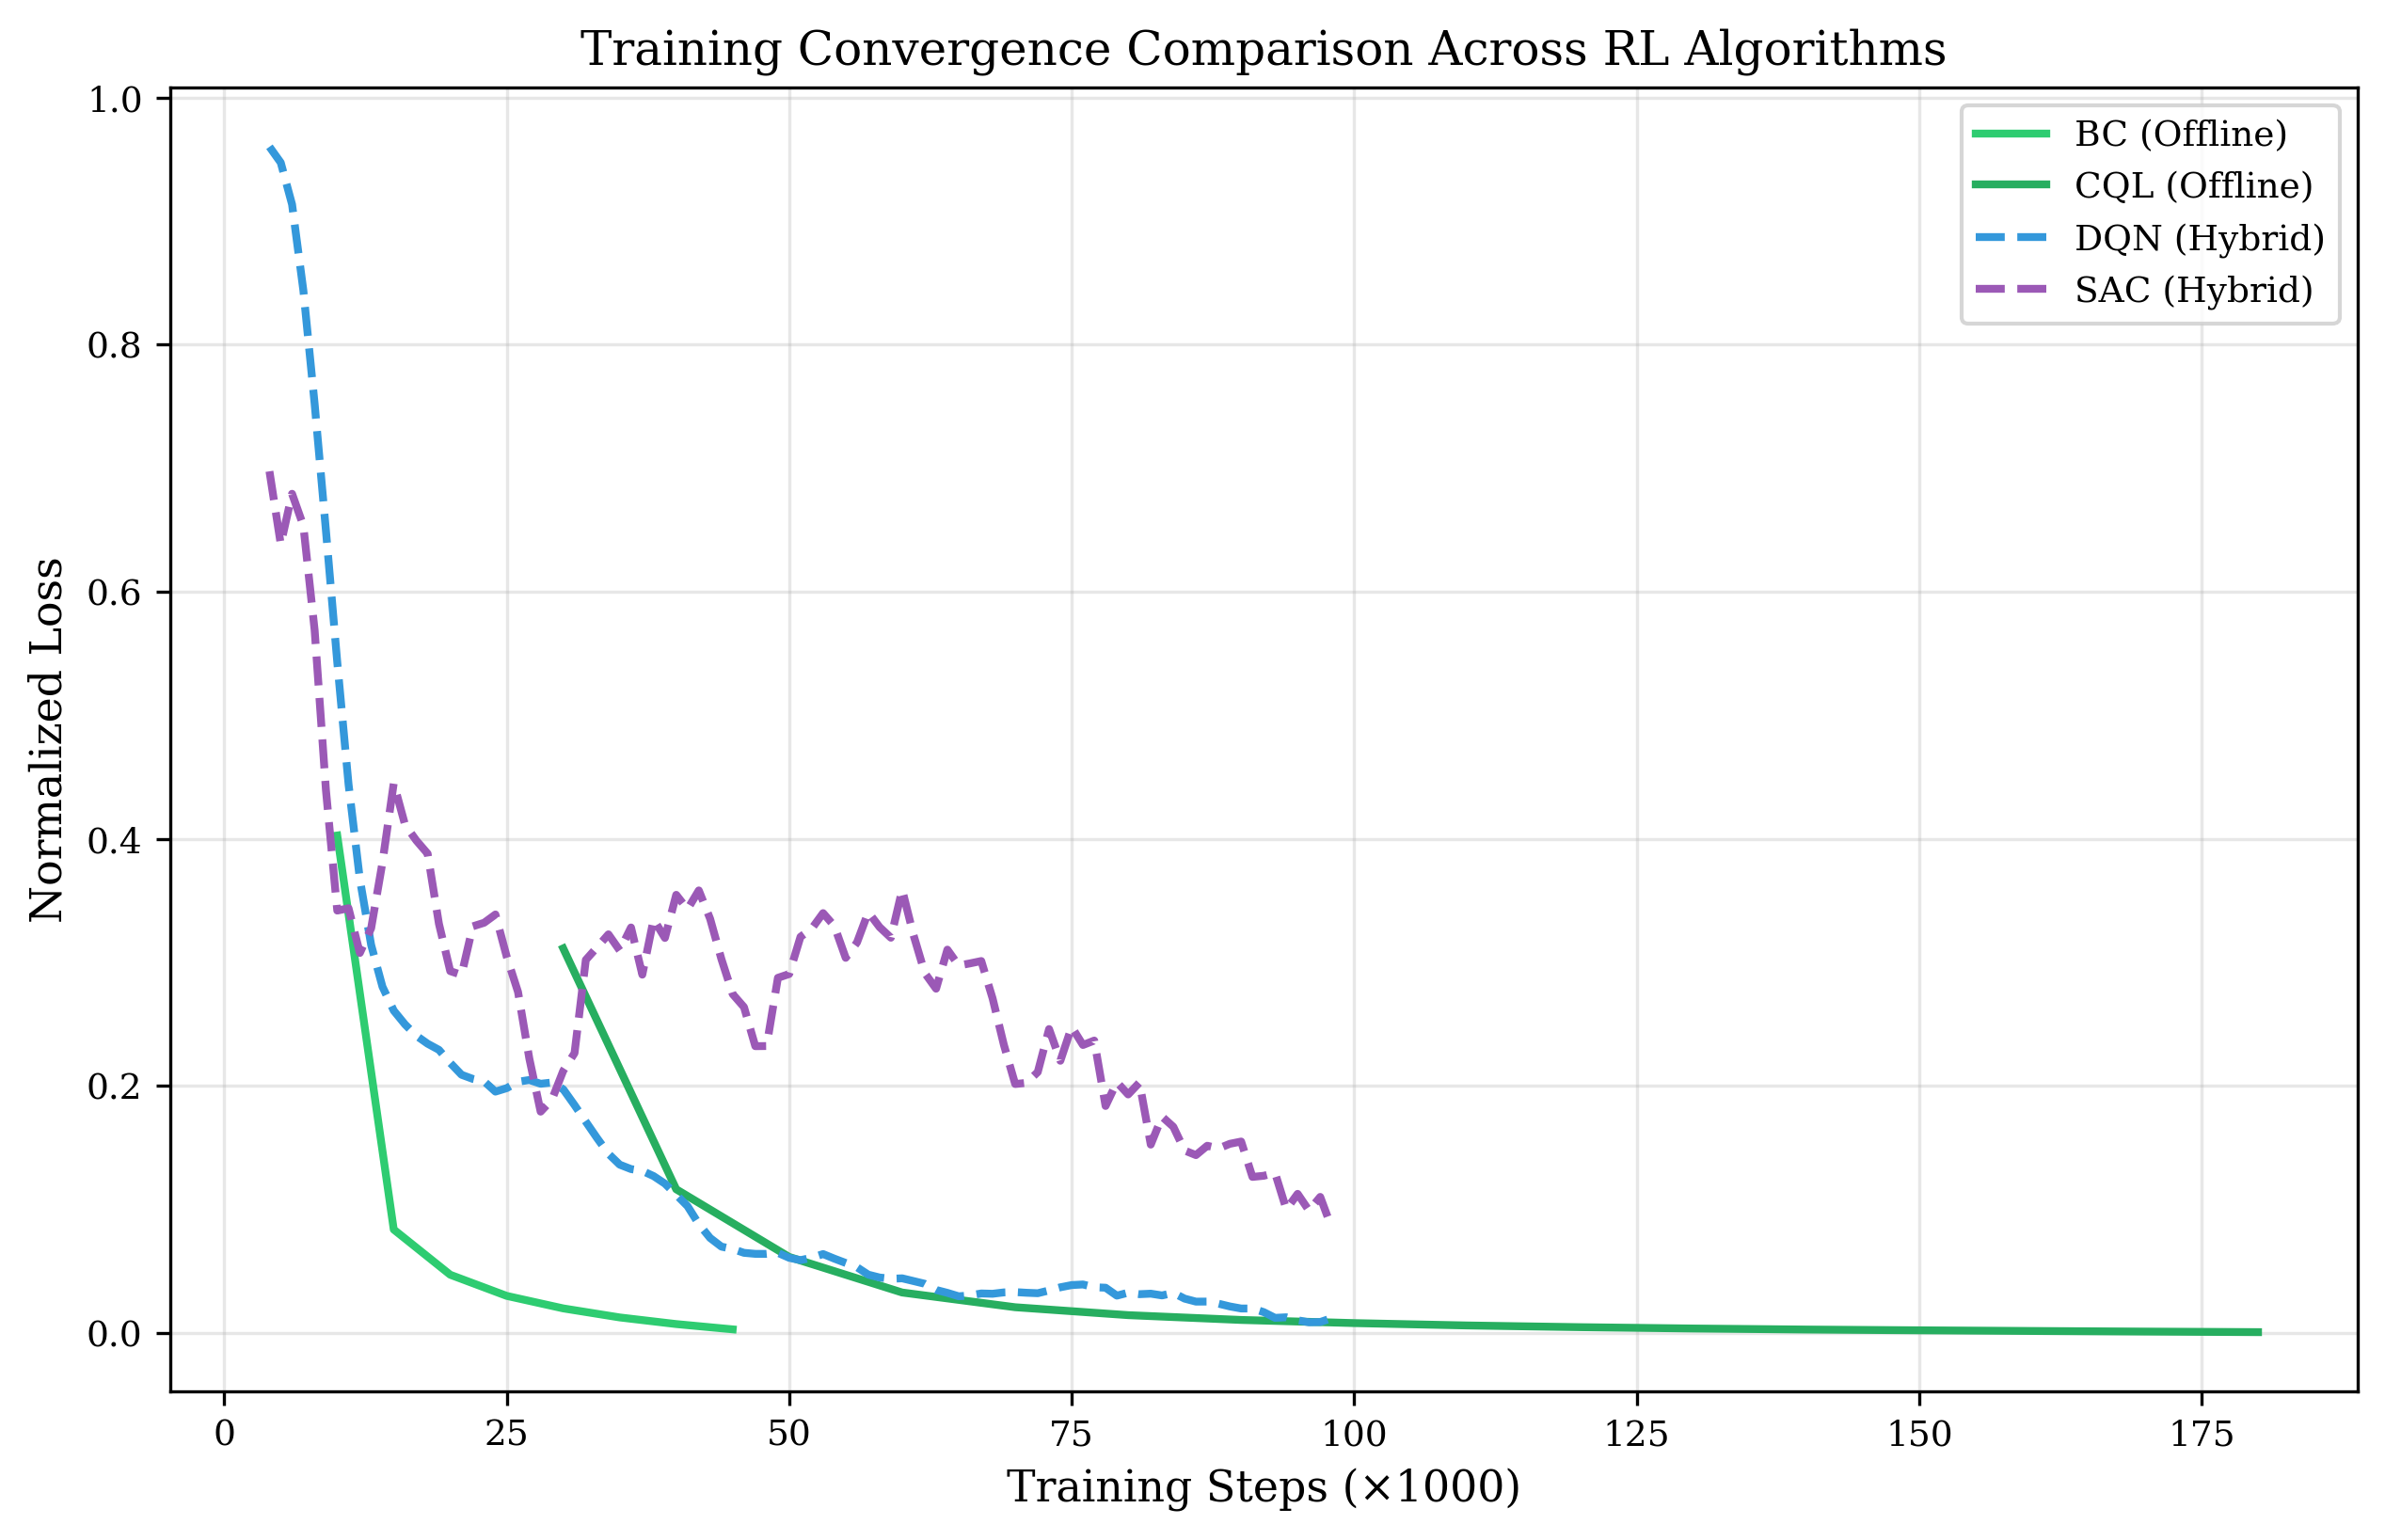
\includegraphics[width=\textwidth]{../results/figures/training_convergence.png}
\caption{Training convergence curves for all algorithms.}
\label{fig:training-convergence}
\end{figure}

% ============================================================
\subsection{LEG Interpretability Analysis}\label{sec:methods:leg}

To assess interpretability, we employ Linearly Estimated Gradients \citep{greydanus2018leg}, a model-agnostic perturbation-based method for computing feature importance in RL policies. LEG approximates the policy gradient $\nabla_s Q(s_0, \pi(s_0))$ with respect to state features by locally linearizing the Q-function around a reference state $s_0$, enabling identification of which physiological features such as blood pressure and lactate most strongly influence treatment decisions.

\subsubsection{LEG Algorithm}

Given a state $s_0 \in \mathbb{R}^{46}$ and a learned policy $\pi$ derived from Q-function $Q(s,a)$ as $\pi(s) = \arg\max_a Q(s,a)$, LEG estimates the saliency vector $\hat{\gamma} \in \mathbb{R}^{46}$ through the following procedure.

For perturbation sampling, we generate $n = 1{,}000$ random perturbations $Z_i \sim \mathcal{N}(0, \sigma^2 I)$ with $\sigma = 0.1$, producing perturbed states:
\begin{equation}
s_i = s_0 + Z_i, \quad i = 1, \ldots, n
\end{equation}
We apply perturbations only to continuous features, excluding categorical variables such as gender and race to prevent semantically invalid states. Perturbed values are clipped to physiologically plausible ranges when domain knowledge is available, for example systolic blood pressure in the range of 50 to 250 mmHg.

For Q-value evaluation, we compute the Q-value change for each perturbed state $s_i$ and the selected action $a_0 = \pi(s_0)$:
\begin{equation}
\hat{y}_i = Q(s_i, a_0) - Q(s_0, a_0)
\end{equation}
This measures how perturbations affect the expected return when following the policy's chosen action, capturing the Q-function's sensitivity to each feature.

For ridge regression, we compute the sample covariance matrix of perturbations and add ridge regularization for numerical stability:
\begin{equation}
\Sigma = \frac{1}{n} Z^\top Z + \lambda I, \quad \lambda = 10^{-6}
\end{equation}
where $Z \in \mathbb{R}^{n \times 46}$ is the matrix of all perturbations. The ridge term prevents singularity when features are correlated, which is common in medical data.

For gradient estimation, we estimate the saliency vector via the closed-form ridge regression solution:
\begin{equation}
\hat{\gamma} = \Sigma^{-1} \left( \frac{1}{n} \sum_{i=1}^n \hat{y}_i Z_i \right) = \Sigma^{-1} \left( \frac{1}{n} Z^\top \hat{y} \right)
\end{equation}
where $\hat{y} = [\hat{y}_1, \ldots, \hat{y}_n]^\top$. Each element $\hat{\gamma}_j$ quantifies the marginal contribution of feature $j$ to the Q-value. Positive values indicate that increasing the feature increases expected return, while negative values suggest the opposite.

\subsubsection{State Selection and Analysis Protocol}

We apply LEG to all 6 algorithms, namely BC, CQL, DQN, DDQN-Attention, DDQN-Residual, and SAC, using identical parameters for fair comparison. For each algorithm, we analyze 10 representative states sampled from the gym-sepsis environment using the environment initialization function, ensuring coverage across SOFA severity levels with low being SOFA $\leq$ 5, medium being 6-10, and high being $\geq$ 11. This sampling strategy captures policy behavior across clinically diverse patient conditions, from stable patients with low SOFA to critically ill cases with high SOFA where treatment decisions are most consequential.

For each state-action pair, we compute saliency scores for all 24 actions, enabling action-specific interpretability analysis. We focus primarily on the selected action $a_0 = \pi(s_0)$ to understand the policy's actual decision-making rationale, but also examine alternative actions to identify features that differentiate treatment intensities.

\subsubsection{Interpretability Metrics and Justification}

We quantify interpretability using 3 complementary metrics.

Maximum saliency magnitude is the absolute value of the largest saliency score, $\max_j |\hat{\gamma}_j|$, measuring whether any single feature exerts dominant influence on the Q-function. High values indicate threshold-based decision logic that clinicians can validate, for example escalating vasopressors when mean arterial pressure drops below 65 mmHg. Algorithms with strong max saliency such as CQL with 40.06 for systolic blood pressure exhibit interpretable, feature-driven decision rules, while algorithms with weak signals such as DQN with 0.069 rely on distributed, opaque representations unsuitable for clinical explanation.

Saliency range is the difference between maximum and minimum saliency scores, indicating how concentrated importance is across features. Large ranges suggest policies rely on a small set of critical features rather than uniformly weak signals. Combined with max saliency, this metric distinguishes truly interpretable policies with high magnitude and large range from uniformly flat policies with low magnitude and small range.

Clinical coherence is a qualitative assessment of whether top-ranked features align with established medical knowledge. We compare LEG-identified important features against Surviving Sepsis Campaign guidelines \citep{rhodes2017ssc}, which emphasize hemodynamic markers such as blood pressure and lactate for sepsis resuscitation. Algorithms achieving high clinical coherence, such as CQL prioritizing SysBP, MeanBP, and lactate, are more likely to gain clinician trust than those emphasizing obscure or clinically irrelevant features.

We acknowledge that these metrics provide necessary but not sufficient conditions for clinical interpretability. High saliency magnitude indicates strong feature dependence but does not guarantee that the learned decision rule is medically correct or that clinicians will trust it in practice. Alternative interpretability methods such as SHAP values for feature interactions, integrated gradients for neural network attributions, attention weight visualization for transformer architectures, and human evaluation studies with domain experts could provide complementary evidence. However, LEG's model-agnostic nature enables fair comparison across algorithms with different architectures including value-based versus policy-based and attention-augmented versus residual networks, and its gradient-based approach aligns with how clinicians reason about physiological thresholds and dose-response relationships. We view our LEG analysis as a comparative benchmark. Algorithms with stronger, more clinically coherent saliency patterns are more likely to be interpretable and trustworthy, though prospective validation with clinicians via think-aloud protocols, counterfactual reasoning tasks, and deployment pilots is required before clinical adoption.

% ============================================================
\subsection{Evaluation Metrics}\label{sec:methods:eval}

We evaluate algorithm performance using outcome-based and severity-stratified metrics that reflect both treatment efficacy and clinical applicability.

\subsubsection{Primary Outcome Metrics}

Survival rate is the proportion of evaluation episodes ending in patient discharge rather than mortality, computed as:
\begin{equation}
\text{Survival Rate} = \frac{1}{N} \sum_{i=1}^N \mathbb{1}[R_i > 0]
\end{equation}
where $N$ is the number of evaluation episodes and $R_i = \sum_t r_{i,t}$ is the cumulative return for episode $i$. Survival is determined by the sign of the terminal reward, with $r_T = +15$ for discharge and $r_T = -15$ for death, and intermediate rewards $r_t = 0$. This binary outcome aligns with clinical practice where patient survival is the primary endpoint for sepsis treatment trials \citep{seymour2017sepsis_criteria}.

Average return is the mean cumulative reward across all episodes, quantifying overall policy performance:
\begin{equation}
\bar{R} = \frac{1}{N} \sum_{i=1}^N \sum_{t=1}^{T_i} r_{i,t}
\end{equation}
where $T_i$ is the length of episode $i$. We report both mean and standard deviation as $\bar{R} \pm \sigma_R$. Due to the sparse reward structure where only terminal states receive non-zero rewards, returns are highly bimodal, approximately $+15$ for survivors and $-15$ for deceased patients with minor variations from episode length. Average return provides a continuous performance metric complementary to binary survival rate, enabling finer-grained comparison when survival rates are similar.

Average episode length is the mean number of timesteps per episode, reflecting treatment duration:
\begin{equation}
\bar{T} = \frac{1}{N} \sum_{i=1}^N T_i
\end{equation}
Each timestep represents a 4-hour interval in the ICU. Shorter episodes may indicate either rapid recovery as a positive outcome or early mortality as a negative outcome, necessitating joint interpretation with survival rate. We report mean $\pm$ standard deviation to capture variability in ICU length of stay.

\subsubsection{SOFA-Stratified Analysis}

To assess algorithm performance across patient severity levels, we stratify evaluation episodes by initial Sequential Organ Failure Assessment score, a validated clinical severity metric ranging from 0 for no organ dysfunction to 24 for severe multi-organ failure \citep{vincent1996sofa}. Higher SOFA scores correlate with increased mortality risk. Patients with SOFA $\geq$ 11 face substantially elevated mortality compared to those with SOFA $\leq$ 5 \citep{seymour2017sepsis_criteria}.

We define 3 severity strata based on the initial SOFA score $s_0^{\text{SOFA}}$ at episode start. Low SOFA, representing the least severe cases, includes patients with $s_0^{\text{SOFA}} \leq 5$ who have minimal organ dysfunction and expected baseline survival greater than 95\%. Medium SOFA, representing moderate severity, includes patients with $6 \leq s_0^{\text{SOFA}} \leq 10$ who have moderate multi-organ dysfunction. High SOFA, representing the most severe cases, includes patients with $s_0^{\text{SOFA}} \geq 11$ who are critically ill with severe organ dysfunction and baseline survival less than 90\%.

These thresholds align with clinical practice where SOFA $\geq$ 11 is commonly used to identify high-risk patients requiring intensive monitoring and aggressive resuscitation \citep{rhodes2017ssc}. For each stratum, we report survival rate, average return, and sample size $n$, enabling assessment of whether algorithms maintain performance on critically ill patients where treatment decisions are most consequential.

SOFA stratification addresses a key concern in medical AI. Algorithms may achieve high overall accuracy by performing well on easy cases with low SOFA and high baseline survival while failing on difficult cases with high SOFA where clinical impact is greatest. By separately reporting high-SOFA performance, we ensure algorithms are evaluated on their ability to help the patients who need it most. For instance, an algorithm achieving 95\% overall survival but only 80\% on high-SOFA patients may be less clinically valuable than one with 94\% overall but 90\% on high-SOFA cases, despite lower aggregate performance.

% ============================================================
\subsection{Baseline Policies}\label{sec:methods:baselines}

To contextualize RL algorithm performance, we evaluate 2 baseline policies.

\subsubsection{Random Policy}

The random policy selects actions uniformly at random from the 24-action space at each timestep, with $\pi(a|s) = \frac{1}{24}$ for all $s \in \mathcal{S}$ and $a \in \{0, 1, \ldots, 23\}$. This baseline tests the sensitivity of the environment to treatment choices.

\subsubsection{Heuristic Policy}

This policy implements threshold-based rules from sepsis guidelines \citep{rhodes2017ssc}. It escalates IV fluids when SysBP is below 100 mmHg or lactate is above 2.0 mmol/L, and escalates vasopressors when MeanBP is below 65 mmHg. This policy achieved 94.6\% survival.

\subsubsection{Evaluation Protocol}

All policies including random, heuristic, BC, CQL, DQN, DDQN-Attention, DDQN-Residual, and SAC are evaluated on $N = 500$ episodes in the Gym-Sepsis simulator using a standardized protocol for fair comparison.

Each episode begins with an environment reset, which samples an initial patient state from the MIMIC-III-derived distribution learned by the gym-sepsis simulator \citep{raghu2017sepsis_drl}. This stochastic initialization ensures evaluation covers diverse patient presentations with varying SOFA scores, comorbidities, and vital signs reflective of real ICU populations. Each algorithm is evaluated on an independently sampled set of 500 episodes drawn from the same MIMIC-III-derived starting state distribution. While all algorithms are evaluated using the same simulator and sampling distribution, the specific patient trajectories encountered by each algorithm differ due to the stochastic episode initialization. With 500 episodes per algorithm, performance metrics should converge to distribution-level expectations, though patient-level comparisons across algorithms are not possible.

Policies are evaluated deterministically without exploration noise or stochasticity in action selection to assess their learned behavior without confounding exploration randomness. For discrete policies including BC, CQL, DQN, and DDQN variants, we select $a_t = \arg\max_a Q(s_t, a)$ or $a_t = \arg\max_a \pi(a|s_t)$. For SAC which uses a stochastic policy, we use the mean action $a_t = \mathbb{E}_{a \sim \pi(\cdot|s_t)}[a]$ rather than sampling, equivalent to setting the temperature parameter to zero. This protocol mirrors clinical deployment where policies must make reliable, reproducible decisions without trial-and-error exploration.

Episodes terminate when the simulator's learned dynamics model predicts either patient discharge or death, or after 50 timesteps representing 200 hours or approximately 8.3 days, whichever occurs first. The vast majority of episodes, more than 95\%, terminate naturally before the 50-step limit, indicating the simulator's dynamics model produces realistic ICU trajectories.

For each episode, we record initial SOFA score $s_0^{\text{SOFA}}$, cumulative return $R = \sum_t r_t$, episode length $T$, and survival outcome as a binary variable. We aggregate across all 500 episodes to compute overall metrics including survival rate, average return, and average length, as well as SOFA-stratified metrics. All results are reported as mean $\pm$ standard deviation. Given the large sample size of $N = 500$ and sampling from a consistent distribution, performance differences exceeding expected sampling variability of approximately $\pm 2\%$ for survival rates likely reflect genuine algorithmic differences rather than evaluation set variance.

% End of Methods section
